\documentclass[15pt, a0paper, portrait]{tikzposter}
\usepackage[utf8]{inputenc}
 
\title{Fast-Slow Dynamics}
\author{Jonna, Kieran, Tom }
\date{14/12/2018}
%\institute{MIGSAA}
 
\usepackage{blindtext}
\usepackage{comment}
\usepackage{amsmath}
%\usepackage{proj1}
\usetheme{Board}
 
\begin{document}
 
\maketitle
 
\block{~}
{

Fast- Slow systems are systems of differential equations that can be viewed on two different time scales, which are separated by a parameter, $\epsilon$. The transition between those two systems is done by a transformation of the time variable $t = \frac{\tau}{\epsilon}$. 
In this project two and three dimensional systems are considered.
Fast System:
\begin{align*} 
x' =&\frac{dx}{dt}= f(x,y,\lambda, \epsilon), \ \ \
y' = \frac{dy}{dt}= \epsilon g( x,y, \lambda, \epsilon),
\\
\epsilon \dot{x} =& \epsilon \frac{dx}{d \tau} = f(x,y,\lambda, \epsilon),\ \ \
\dot{y} = \frac{dy}{d \tau} =  g( x,y, \lambda, \epsilon),
\end{align*}
}
\block{~}
{\textbf{Motivation and Setup}\\ \centering
    \begin{tabular}{p{0.7\linewidth}p{0.3\linewidth}}
    {Fast- Slow systems are systems of differential equations that can be viewed on two different time scales, which are separated by a parameter, $\epsilon$. The transition between those two systems is done by a transformation of the time variable $t = \frac{\tau}{\epsilon}$. 
In this project two }&{
    $
    \begin{cases}
   x' &= \frac{dx}{dt}= f(x,y,\lambda, \epsilon), \\
   y' &= \frac{dy}{dt}= \epsilon g( x,y, \lambda, \epsilon)
    \end{cases}\label{FastS}
    $}\\ 
{and three dimensional systems are considered.}&
{$    \begin{cases}
    \epsilon \dot{x} &= \epsilon \frac{dx}{d \tau} = f(x,y,\lambda, \epsilon),\\
    \dot{y} & = \frac{dy}{d \tau} =  g( x,y, \lambda, \epsilon),
    \end{cases}\label{SlowS}
    $ }
\end{tabular}
} 



\begin{columns}
    \column{0.5}
    \block{Van der Pol System}
{Fast System:
\begin{equation*}\label{fastsystem}
    \begin{cases} x'=y-\frac{x^3}{3}+x\\
    y'=-\epsilon x,
    \end{cases}
\end{equation*}
Slow System: 
\begin{equation*}\label{slowsystem}
    \begin{cases} \epsilon \dot{x}=y-\frac{x^3}{3}+x\\
    \dot{y}=-x,
    \end{cases}
\end{equation*}
}

%   
\colorlet{blockbodybgcolor}{green!60}
\block{Phase Portrait: Van der Pol System}
{
	 
	\begin{tikzfigure}[h!]
		\centering
		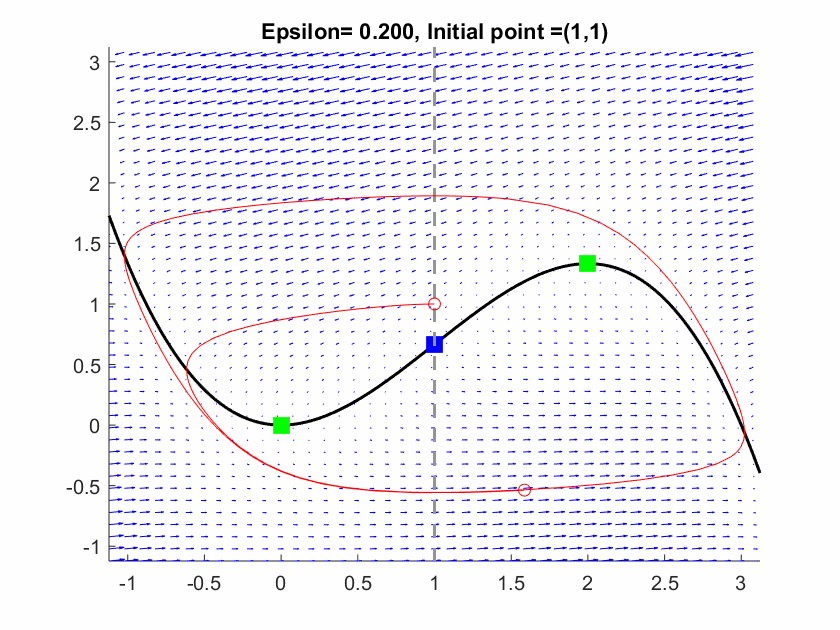
\includegraphics[height=10cm,width=13cm]{Posterpic1.jpg}
		%\caption{The reduced flow where a) $\lambda=0$ and b) $\lambda>0$.}
		%label{fig: Canard Point}
	\end{tikzfigure}
}
\column{0.5}
\block{Canard Cycle}
{
	Layer Problem:
	\begin{equation*}\label{fastsystem0}
	\begin{cases} x'=y-\frac{x^3}{3}+x,\\
	y'=0,
	\end{cases}
	\end{equation*}
	Reduced Problem:
	\begin{equation*}\label{slowsystem0}
	\begin{cases} 0=y-\frac{x^3}{3}+x:=f,\\
	\dot{y}=-x.
	\end{cases}
	\end{equation*}
	
}

    \block{Phase Portrait: Canard Cycle}
{
	\begin{tikzfigure}[h!]
		\centering
		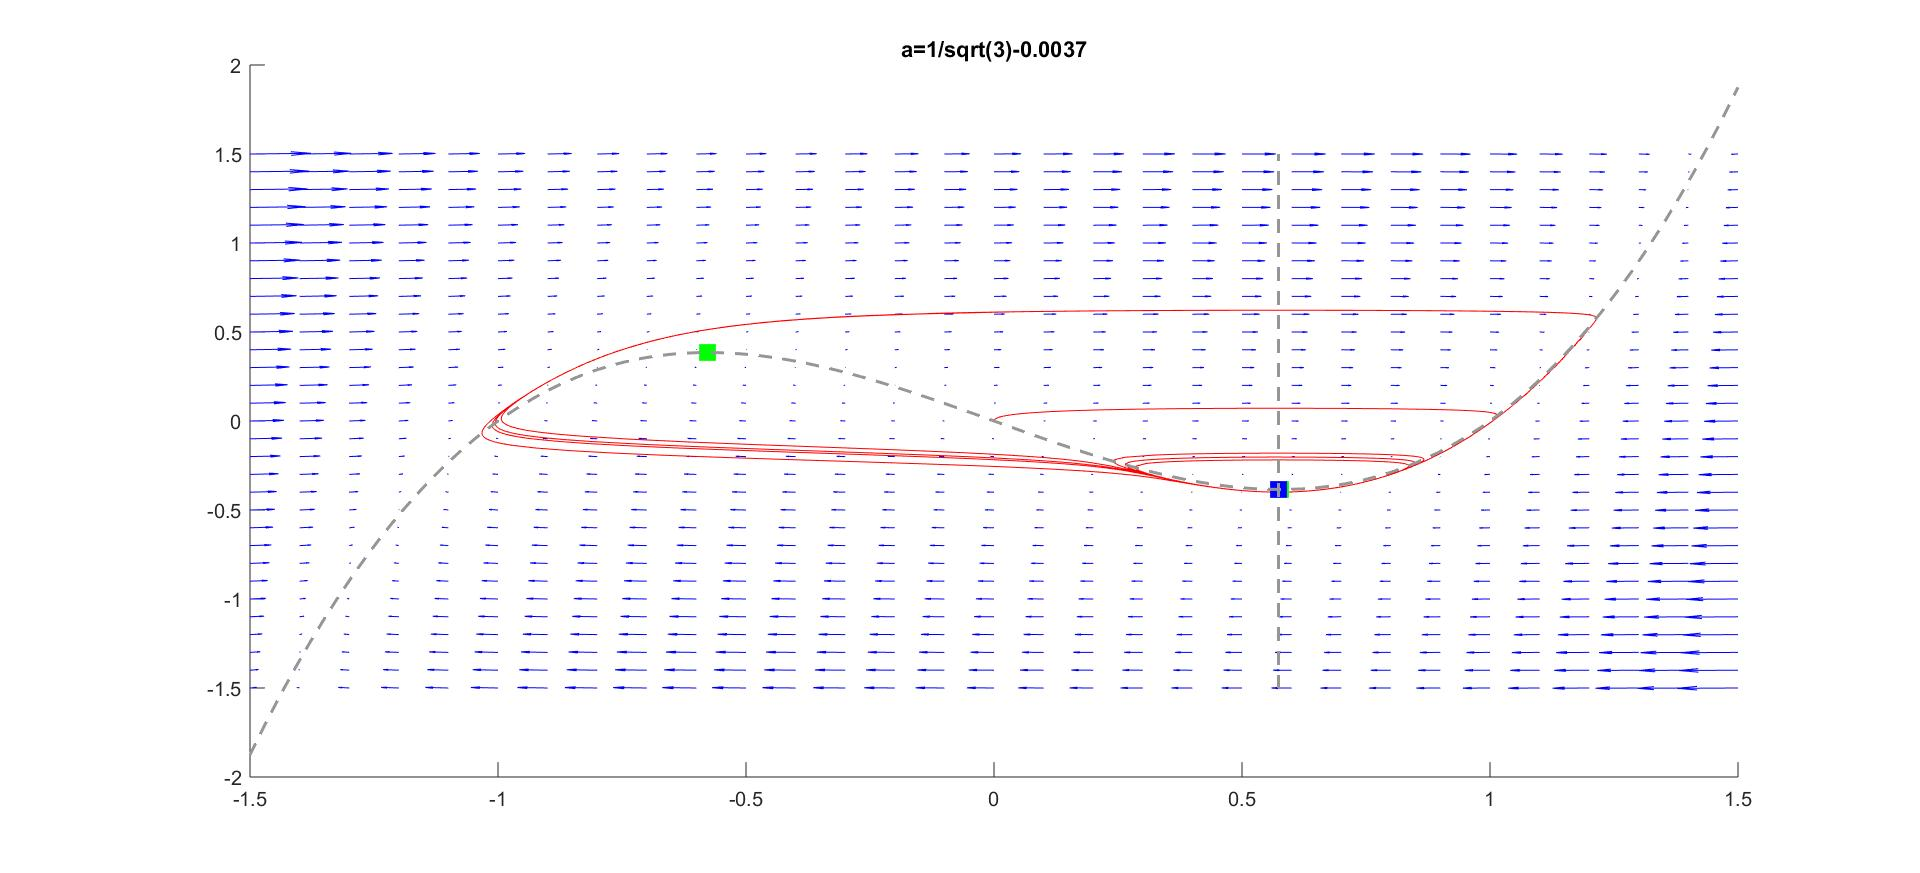
\includegraphics[height=10cm,width=13cm]{../Code/behaviourswitch}
		%\caption{The reduced flow where a) $\lambda=0$ and b) $\lambda>0$.}
		%label{fig: Canard Point}
\end{tikzfigure}}

\end{columns}
%%%%%%%%%%%%%%%%%%%%%%%%%%%%%%%%
%%%%%%%%%%%%%%%%%%%%%%%
%%%%%%%%%%%%%%
%%%%%%%%
\block{~}
{\textbf{Blow-up}\centering
	
	Fast- Slow systems are systems of differential equations that can be viewed on two different time scales, which are separated by a parameter.
	These systems are generally of the form
	\begin{equation*} 
	\begin{cases}
	x' &=\frac{dx}{dt}= f(x,y,\lambda, \epsilon),\\
	y' &= \frac{dy}{dt}= \epsilon g( x,y, \lambda, \epsilon),
	\end{cases}\label{FastS}
	\end{equation*}
	which is known as the fast system.
	Using a scaling for the time, $t = \frac{\tau}{\epsilon} $, we find that this can be rewritten as
	\begin{align*}
	\begin{cases}
	\epsilon \dot{x} &= \epsilon \frac{dx}{d \tau} = f(x,y,\lambda, \epsilon),\\
	\dot{y} & = \frac{dy}{d \tau} =  g( x,y, \lambda, \epsilon),
	\end{cases}\label{SlowS}
	\end{align*}
	which is called the slow system.
}
\begin{columns}
\column{0.5}
\colorlet{blockbodybgcolor}{green!60}
\block{Phase Portrait: Van der Pol System}
{
	
	\begin{tikzfigure}[h!]
		\centering
		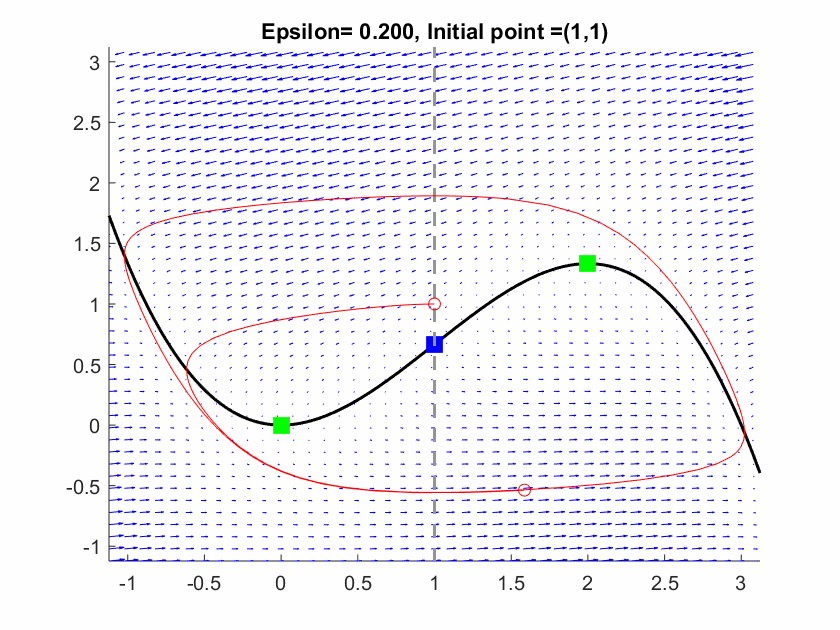
\includegraphics[height=10cm,width=13cm]{Posterpic1.jpg}
		%\caption{The reduced flow where a) $\lambda=0$ and b) $\lambda>0$.}
		%label{fig: Canard Point}
	\end{tikzfigure}
}
	\column{0.5}
   \block{Phase Portrait: Singular Limit}
{
	\begin{tikzfigure}[h!]
		\centering
		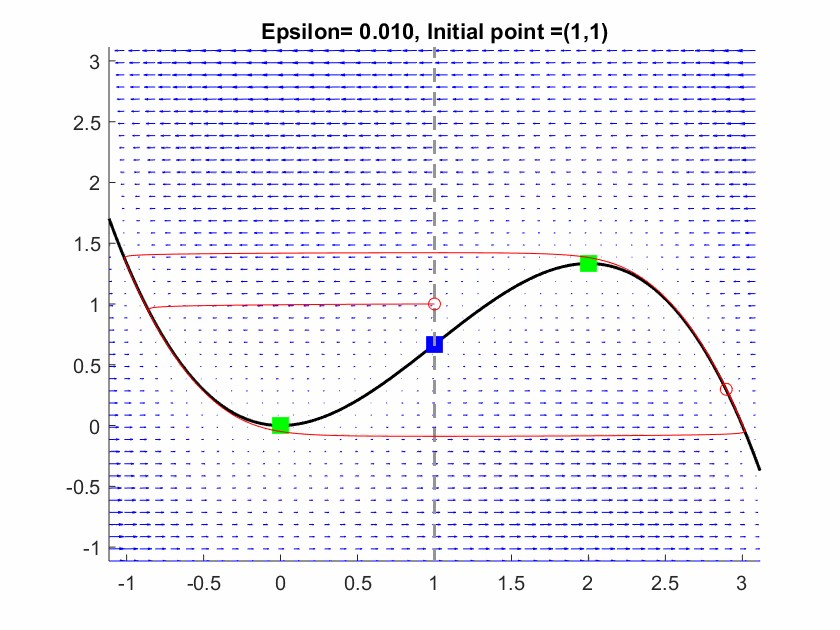
\includegraphics[height=10cm,width=13cm]{Posterpic2.jpg}
		%\caption{The reduced flow where a) $\lambda=0$ and b) $\lambda>0$.}
		%label{fig: Canard Point}
\end{tikzfigure}}
\end{columns}


%%%%%%%%%%%%%%%%%%%%%%%%%%%%%%%%%%%%%%%%%%%%%%%%%%%%%%%%%%
%%%%%%%%%%%%%%%%%%%%%%%%%
%%%%%%%%%%%%%%
\block{~}
{\textbf{Mixed-Mode Oscillations}\centering
	In the planar case, canards only occure within $O(\epsilon)$ of the fold point. To get more readily observable canards, another variable is introduced.
	
	\begin{align*} \dot{x} = y-x^2-x^3,\qquad \dot{y} = \epsilon(z-x),\qquad\dot{z}= \epsilon(-\nu-ax-by-cz) \end{align*}
}
\begin{columns}
	\column{0.5}
	\colorlet{blockbodybgcolor}{green!60}
	\block{Phase Portrait: Van der Pol System}
	{
		
		\begin{tikzfigure}[h!]
			\centering
			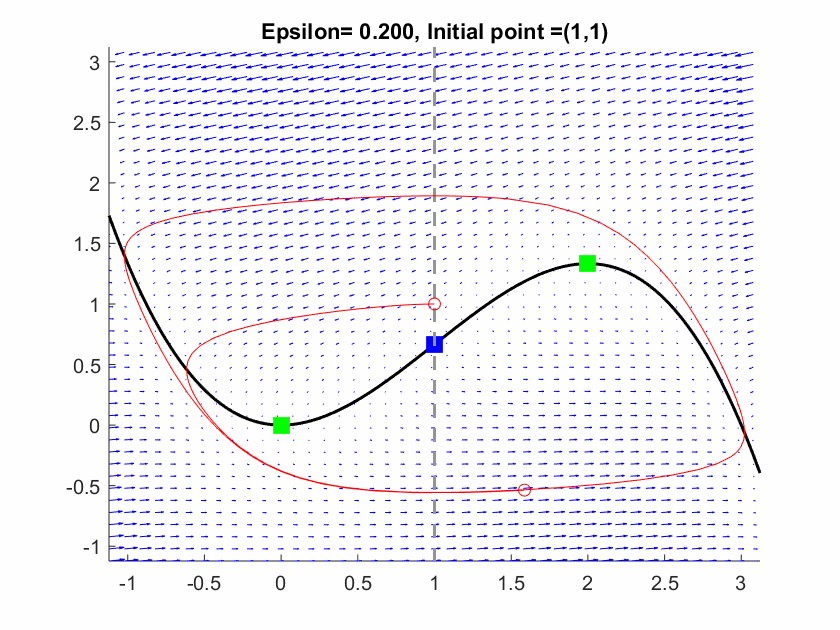
\includegraphics[height=10cm,width=13cm]{Posterpic1.jpg}
			%\caption{The reduced flow where a) $\lambda=0$ and b) $\lambda>0$.}
			%label{fig: Canard Point}
		\end{tikzfigure}
	}
	\column{0.5}
	\block{Phase Portrait: Singular Limit}
	{
		\begin{tikzfigure}[h!]
			\centering
			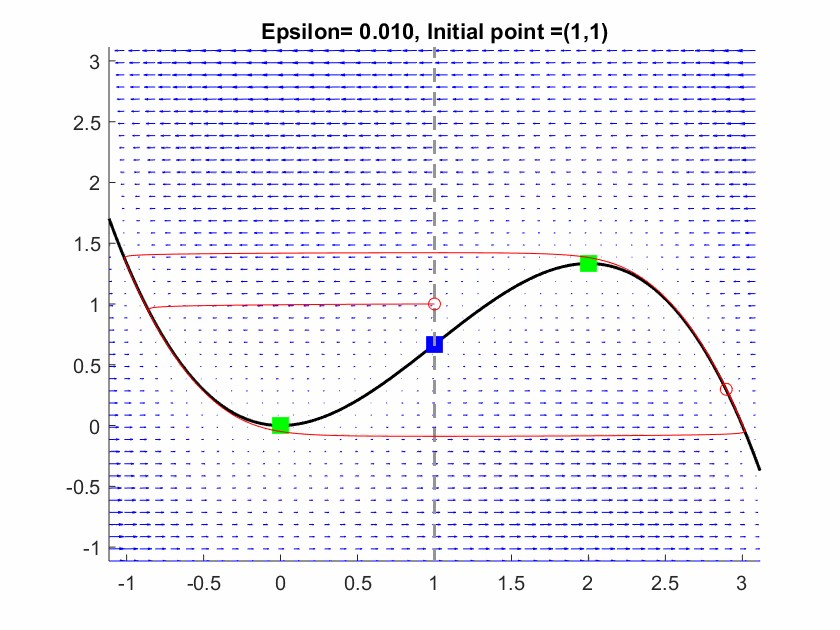
\includegraphics[height=10cm,width=13cm]{Posterpic2.jpg}
			%\caption{The reduced flow where a) $\lambda=0$ and b) $\lambda>0$.}
			%label{fig: Canard Point}
	\end{tikzfigure}}
\end{columns}




\end{document}